\documentclass[aspectratio=169,12pt]{beamer}

\usepackage[english]{babel}
\usepackage{minted}
\usepackage{textcomp}
\usepackage{subcaption}

\usepackage{tikz}
\usepackage{pgfplots}
\usetikzlibrary{positioning,fit,calc}
\tikzset{box/.style={draw,text width=3cm,minimum height=2cm,align=center,rounded corners=.25cm}}
\tikzset{ar/.style={->,>=latex}}
\tikzset{dar/.style={dashed,->,>=latex}}


\usepackage{array}
\usepackage{booktabs}
\usepackage{threeparttable}
\usepackage{wasysym}

\usepackage{hyperref}

\usetheme{metropolis}

\title{Using Prometheus to monitor your build pipelines}
\subtitle{CfgMgmtCamp 2019}
\author{Lander Van den Bulcke -- Open Source Consultant @ Inuits}
\date{}
\institute{landervdb @ \{twitter,github,freenode\}}

\begin{document}

\maketitle

\begin{frame}{Pipelines...}
  \begin{center}
    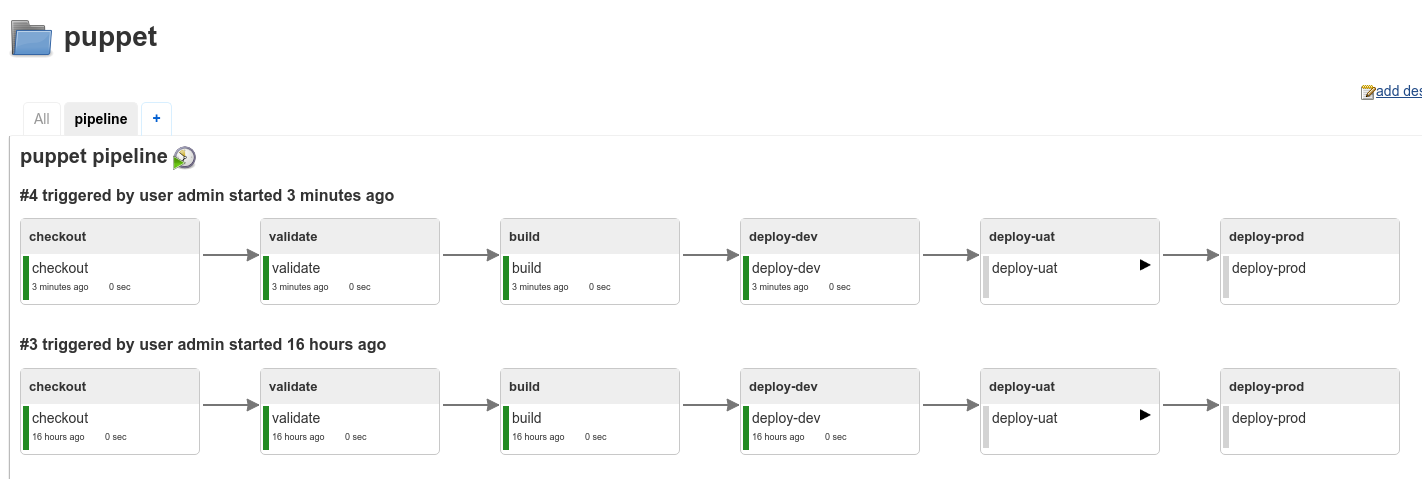
\includegraphics[width=\textwidth]{img/pipeline.png}
  \end{center}
\end{frame}

\begin{frame}[fragile]{Problem}
  \begin{center}
    We do promotions from \textit{DEV} $\rightarrow$ \textit{UAT} $\rightarrow$ \textit{PROD} manually. \\
    \vspace{20pt}
    Problem: people seem to forget to click this button...
  \end{center}
\end{frame}

\begin{frame}[fragile]{Solution?}
  \begin{center}
    Let's monitor this stuff! \\
    \vspace{20pt}
    Let's use Prometheus, there's an exporter for that! \\
    \vspace{20pt}
    \url{https://github.com/lovoo/jenkins_exporter}
  \end{center}
\end{frame}

\begin{frame}[fragile]{Problem (bis)}
  \begin{center}
    Uses the Jenkins JSON API \\
    \vspace{20pt}
    Does \textit{at least} 1 HTTP request for every job \\
    \vspace{20pt}
    We have around 2500 jobs in or main Jenkins master \\
    \vspace{20pt}
    \textbf{\textit{Great} if you want to DOS your Jenkins master!}
  \end{center}
\end{frame}

\begin{frame}[fragile]{Solution (bis)!}
  \begin{center}
    \Large\textbf{I'll just write my own!} \\ 
    
\includegraphics[scale=0.3]{img/go.png}\\
    \normalsize Parse Jenkins config directly \\
    \vspace{10pt}
    Concurrent \\ 
    \vspace{10pt}
    Add custom metrics!
  \end{center}
\end{frame}

\begin{frame}[fragile]{Assumptions}
  \begin{center}
    \textit{Build Environment} plugin installed \\
    \vspace{20pt}
    Your pipelines all follow the same patterns
  \end{center}
\end{frame}

\begin{frame}[fragile]{Assumptions: folder structure}
  \begin{minted}{text}
/
├── folder
│   ├── subfolder
│   │   ├── checkout
│   │   ├── validate
│   │   ├── ...
│   │   ├── deploy-dev
│   │   └── deploy-prod
│   └── ...
└── ...
  \end{minted}
\end{frame}

\begin{frame}{Frustration :(}
  \begin{center}
    Sooo... Jenkins decided to switch to XML 1.1 \\
    \vspace{20pt}
    Go XML parser doesn't support this... \\
    \vspace{20pt}
    Dirty hacking required for now :(
  \end{center}
\end{frame}

\begin{frame}[fragile]{Results?}
  So what does this give us?
  \begin{minted}[fontsize=\scriptsize,breaklines]{text}
# HELP jenkins_last_build_duration_seconds Duration of the last build
# TYPE jenkins_last_build_duration_seconds gauge
jenkins_last_build_duration_seconds{folder="pipelines/puppet", jenkins_job="checkout", result="stable"} 0.029
jenkins_last_build_duration_seconds{folder="pipelines/puppet", jenkins_job="checkout", result="successful"} 0.029
...
# HELP jenkins_last_build_number Build number of the last build
# TYPE jenkins_last_build_number gauge
jenkins_last_build_number{folder="pipelines/puppet", jenkins_job="checkout", result="stable"} 4
jenkins_last_build_number{folder="pipelines/puppet", jenkins_job="checkout", result="successful"} 4
...
  \end{minted}
\end{frame}

\begin{frame}[fragile]{But what can I do with it?}
  \begin{minted}[fontsize=\scriptsize,breaklines]{yaml}
 - record: jenkins:job:duration:avg7d
   expr: avg_over_time(jenkins_last_build_duration_seconds[7d])
 - alert: JobLongExecution
   expr: jenkins_last_build_duration_seconds > 1.2 * jenkins:job:duration:avg7d
   labels:
     severity: warning
   annotations:
     summary: "Execution of last {{ $labels.result }} build for {{ $labels.jenkins_job }} job in folder {{ $labels.folder }} took unusually long"
  \end{minted}
\end{frame}

\begin{frame}[fragile]{Something more useful?}
  \begin{minted}[fontsize=\scriptsize,breaklines]{yaml}
 - record: jenkins:deploytimedelta:devprod
   expr: jenkins_last_build_timestamp_seconds {result="successful",jenkins_job="deploy-dev"} - ignoring(jenkins_job) jenkins_last_build_timestamp_seconds {result="successful",jenkins_job="deploy-prod"}
 - alert: LongTimeSinceDeployToPROD
   expr: jenkins:deploytimedelta:devprod > 300
   labels:
     severity: warning
   annotations:
     summary: "The build for {{ $labels.folder }} on PROD is at least 5 minutes older than the one on DEV"
  \end{minted}
\end{frame}

\begin{frame}[fragile]{Problems (again?!)}
  \begin{center}
    \Large What if we trigger a promote on an older version?
  \end{center}
\end{frame}

\begin{frame}[fragile]{Solution!}
  \begin{center}
    \large Custom metrics! \normalsize \\
    \vspace{20pt}
    \verb|CHECKOUT_BUILD_NUMBER|\\
    $\Downarrow$ \\
    \verb|jenkins_custom_last_checkout_build_number|
  \end{center}
\end{frame}

\begin{frame}[fragile]{Finally something we can work with!}
  \begin{minted}[fontsize=\scriptsize,breaklines]{yaml}
 - record: jenkins:deploydelta:devprod
   expr:  jenkins_custom_last_checkout_build_number {result="successful",jenkins_job="deploy-dev"} - ignoring(jenkins_job) jenkins_custom_last_checkout_build_number {result="successful",jenkins_job="deploy-prod"}
 - alert: BigVersionDifferencePROD
   expr: jenkins:deploydelta:devprod > 3
   labels:
     severity: warning
   annotations:
     summary: "The build for {{ $labels.folder }} on PROD is at least 3 versions  older than the one on DEV"
  \end{minted}
\end{frame}

\begin{frame}{Dashboards!}
  \begin{center}
    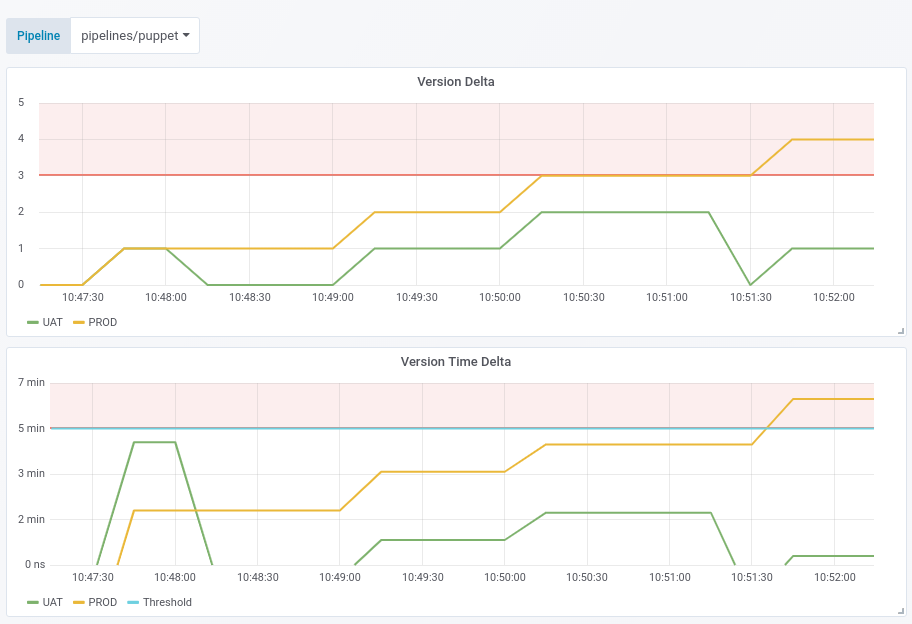
\includegraphics[width=0.8\textwidth]{img/graphs.png}
  \end{center}
\end{frame}

\begin{frame}{Dashboards!}
  \begin{center}
    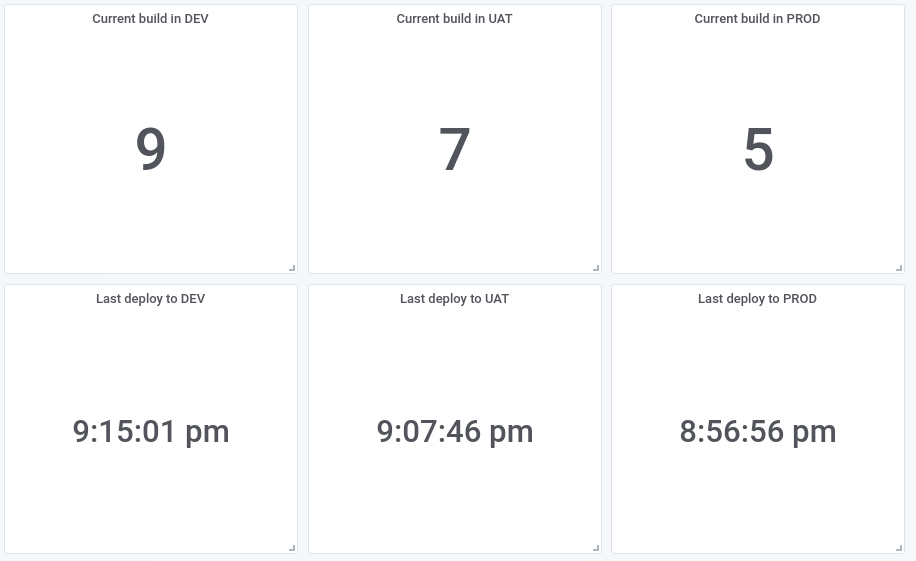
\includegraphics[width=0.8\textwidth]{img/stats.png}
  \end{center}
\end{frame}

\begin{frame}{Dashboards!}
  \begin{center}
    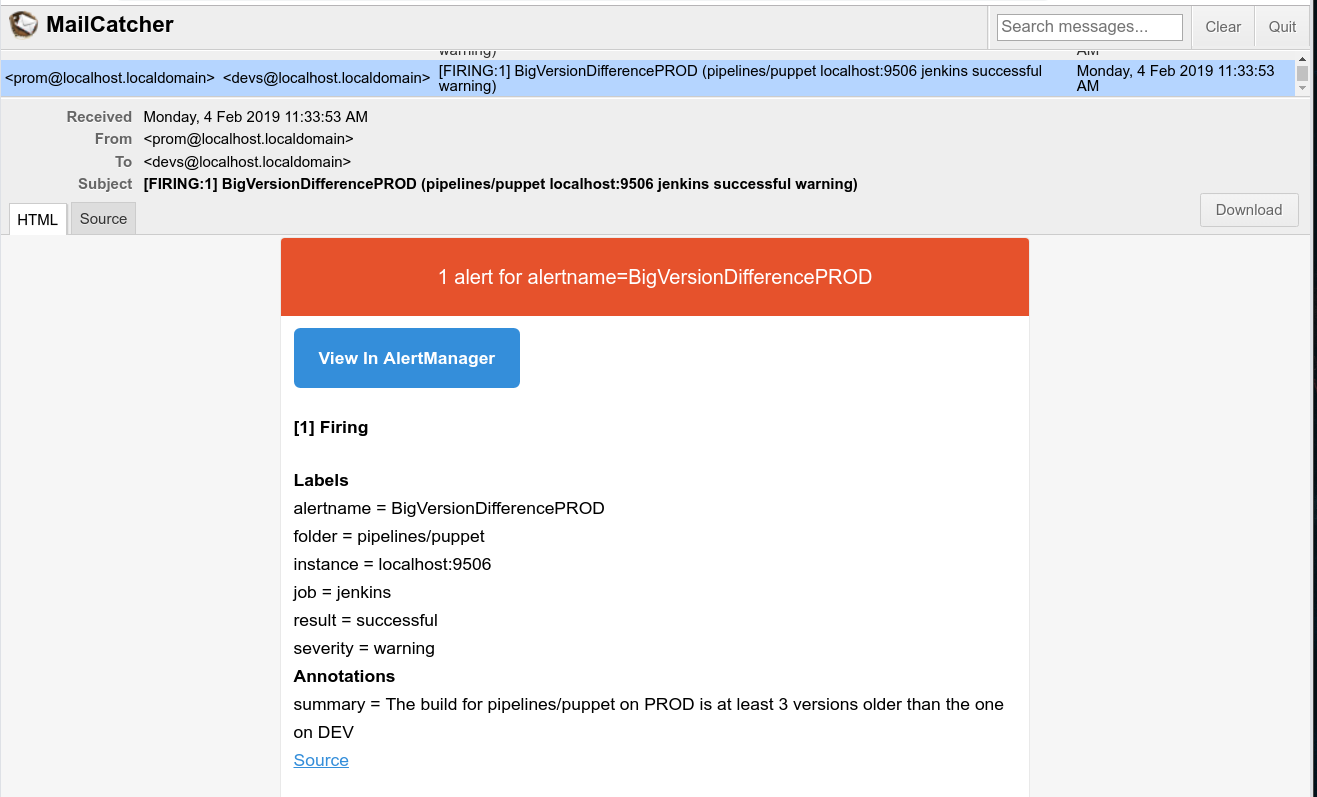
\includegraphics[width=0.8\textwidth]{img/alerts.png}
  \end{center}
\end{frame}

\begin{frame}[fragile]{Find out more}
  \begin{center}
    Use it! Fork it! \\ 
    \url{https://github.com/landervdb/jenkins_exporter} \\ 
    \vspace{20pt}
    Configuration used in this presentation: \\
    \url{https://git.io/fhSUV}
  \end{center}
\end{frame}

\begin{frame}[standout]
  kthxbye
\end{frame}

\end{document}
